\documentclass[12pt]{article}

\usepackage{amssymb,amsmath,amsthm}
\usepackage{graphicx}
%\usepackage{fullpage}
\usepackage[final,colorlinks,hyperindex,unicode=true]{hyperref}
%\usepackage{tikz}
\usepackage{pgfplots}
\usepackage[shadow,colorinlistoftodos,textwidth=4cm]{todonotes}

\newcommand{\jpgpic}[1]{\begin{center}\includegraphics[width=\textwidth]{#1.jpg}\end{center}}

\begin{document}
\author{M. Dvorkin, A. Kulikov}
\title{A Bruijn Graph Approach}
%\date{March 14, 2011}
\maketitle

\listoftodos
\tableofcontents

\newpage

\section{General Idea}

The main goal of this approach is to simplify a \emph{de Bruijn} graph
constructed on a given set of reads while still preserving 
``the structure'' of the graph. Namely, instead 
of representing each read as a sequence of edges 
between its consecutive $k$-mers (in which case a read of length $r$ defines
$r-k-1$ edges) we represent it as just one (or a few, in general)
edge between some of its $k$-mers. For example, for 
reads {\tt ACGTACT} and {\tt TACTAGC} and $k=3$
instead of all gray edges in the figure below we will have 
only two black edges.
\begin{center}
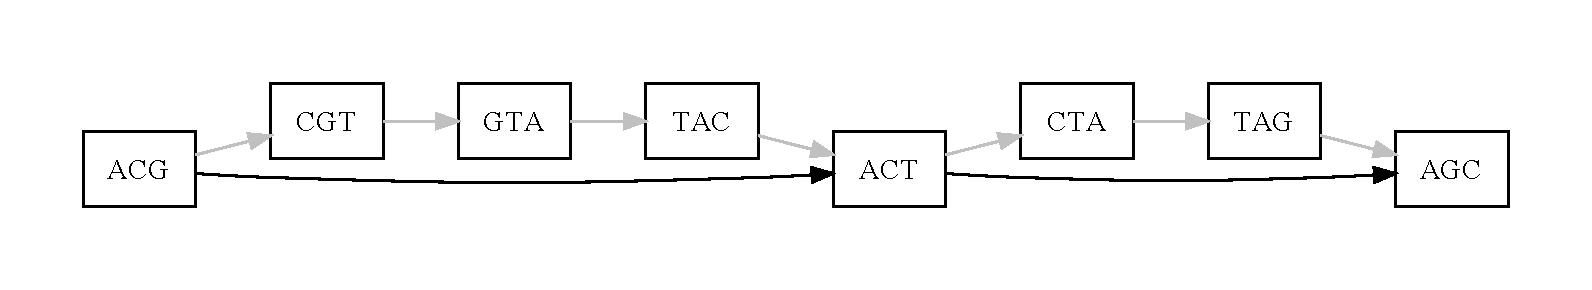
\includegraphics[width=\textwidth]{fig1.pdf}
\end{center}
The hope is that the resulting graph will be easier to handle 
and at the same time it will have essentially the same structure 
as the original de Bruijn graph.{\todo{we should probably cite the paper 
on minimizers and use the word `minimizer' instead of `earmarked $k$-mer'?..}}

\subsection{Example}

\begin{figure}
\caption{De Bruijn (grey) and A Bruijn (black) graphs of genomes {\tt ACTGACTGTTGACACTG} ($readsize=9$, $k=5$)
and {\tt ATTGGTACATTGTGGTACGTACTGACT} ($readsize=11$, $k=5$).}\label{fig23}
\begin{center}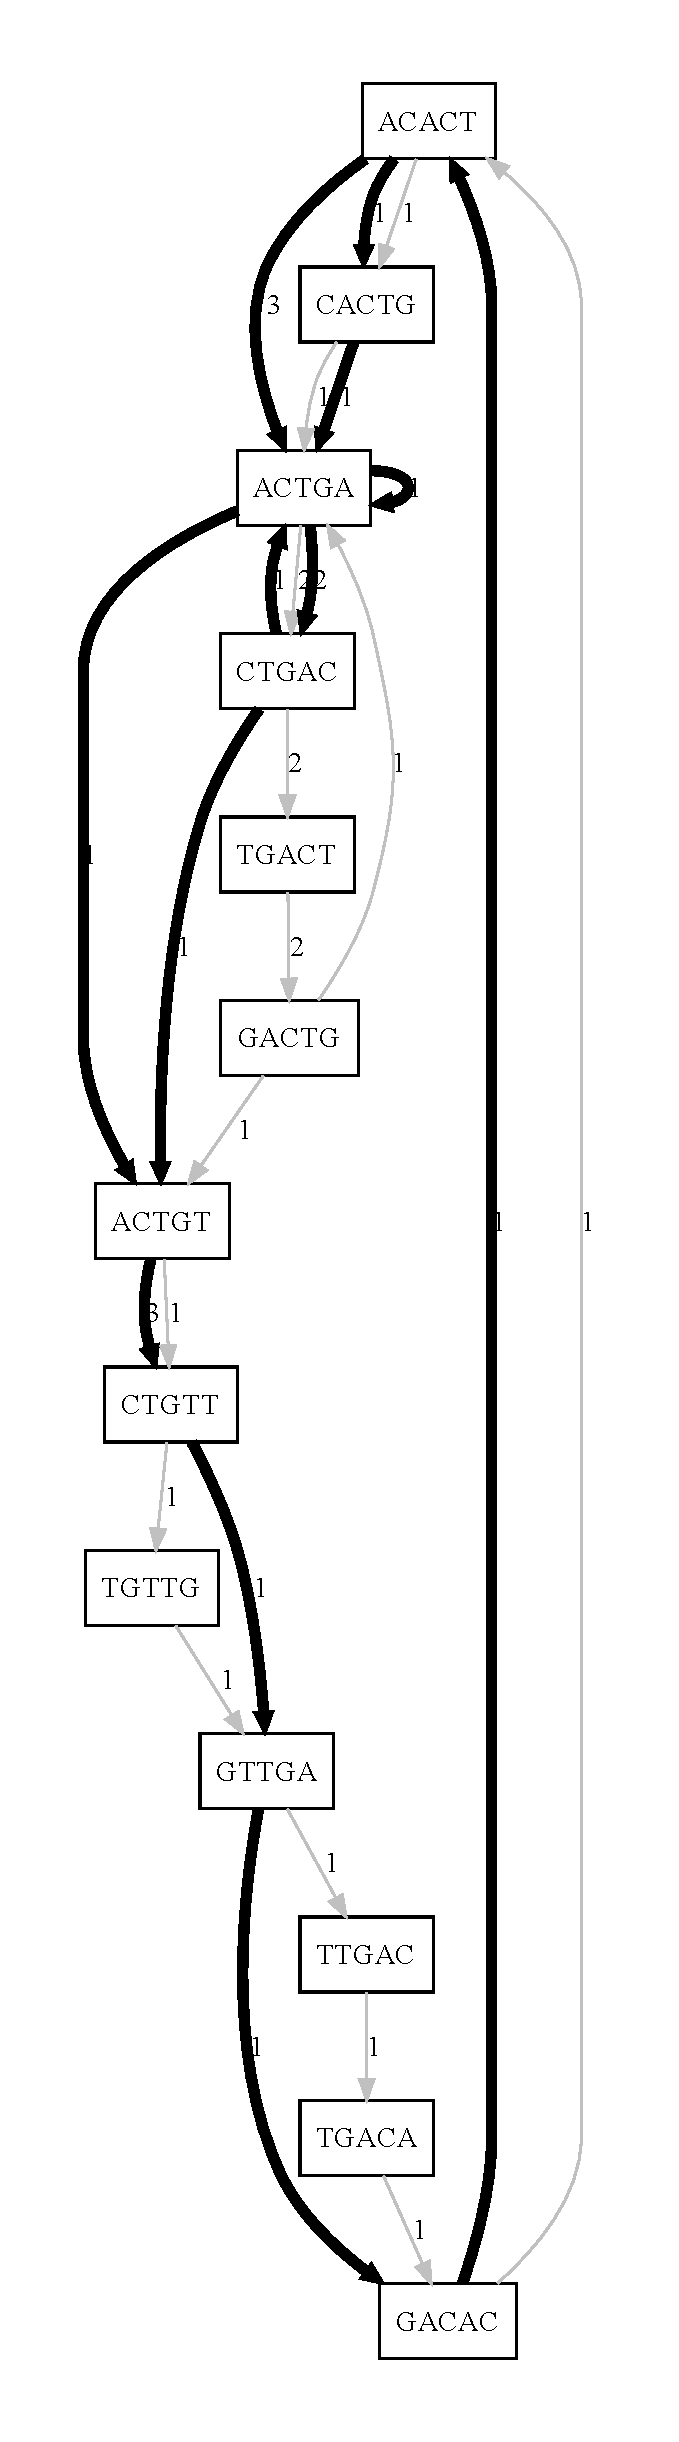
\includegraphics[height=0.9\textheight]{fig2.pdf}
~~~~~~~~~~~~~~
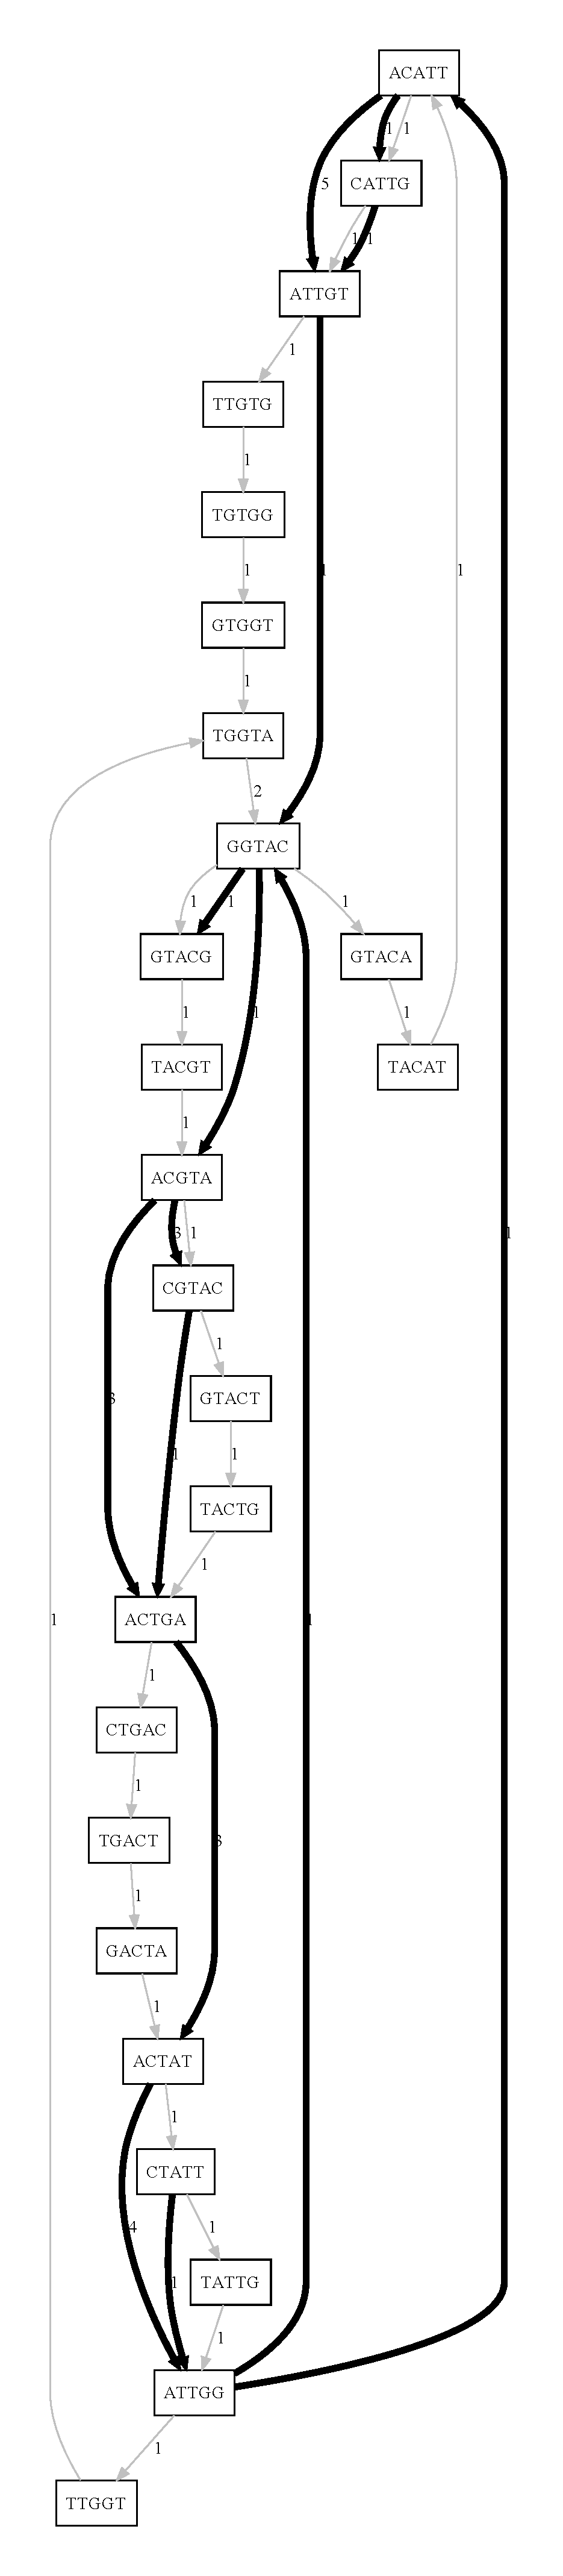
\includegraphics[height=0.9\textheight]{fig3.pdf}\end{center}
\end{figure}

Fig.~\ref{fig23} shows de Bruijn (black edges) and A Bruijn (grey edges) graphs for two toy genomes 
{\tt ACTGACTGTTGACACTG} and {\tt ATTGGTACATTGTGGTACGTACTGACT}. Numbers on edges are their multiplicities. 
We assume that the genome is circular and that we are given the set of all its reads.


\subsection{Advantages of A Bruijn graph over de Bruijn graph}
\begin{enumerate}
\item Clearly, it requires less memory.
\item In general, we expect that the resulting A Bruijn graph 
will have the same structure as the corresponding condensed de Bruijn graph.
If so, this would allow us to construct the condensed de Bruijn graph
using less time and memory.
\item If the used hash-function respects frequency of $k$-mers
the resulting graph will contain a smaller fraction of erroneous $k$-mers.
\item If the hash function does not mark $k$-mers that appear too often, then 
some of the repeats will be already resolved in A Bruijn graph.

An example of this effect is given in Fig.~\ref{fig:different_orderings}
where two A Bruijn graphs of a genome {\tt TAAACGAAAC} ($readsize=6$, $k=3$) 
are shown. The difference is in the way $3$-mers are ordered. Green edges 
correspond to the standard lexicographic ordering ({\tt AAA}$<${\tt 
AAC}$<\dots<${\tt TTT}). Now note that the considered genome contains a 
repeat {\tt AAAC}. Assume that the hash function treats $3$-mers {\tt AAA}
and {\tt AAC} from this repeat as maximal. Namely, let the ordering be the 
following:
\[{\tt TAA}<{\tt ACG}<{\tt CGA}<{\tt GAA}<{\tt CTA}<{\tt ACT}<{\tt AAA}<{\tt AAC} \, .\]
As figure shows, this ordering gives a graph consisting of just one cycle.
A slightly more complicated example is given on Fig.~\ref{fig:different_orderings2}.
There, the corresponding genome {\tt ATGCATTGCACTGCA} contains a repeat {\tt TGCA}
three times. Hence de Bruijn graph spells at least two different genomes. 
%By a careful choice of 


\begin{figure}
\caption{A Bruijn graphs of genome {\tt TAAACGAAAC} ($readsize=6$, $k=3$)
for different orderings on $3$-mers.}\label{fig:different_orderings}
\begin{center}
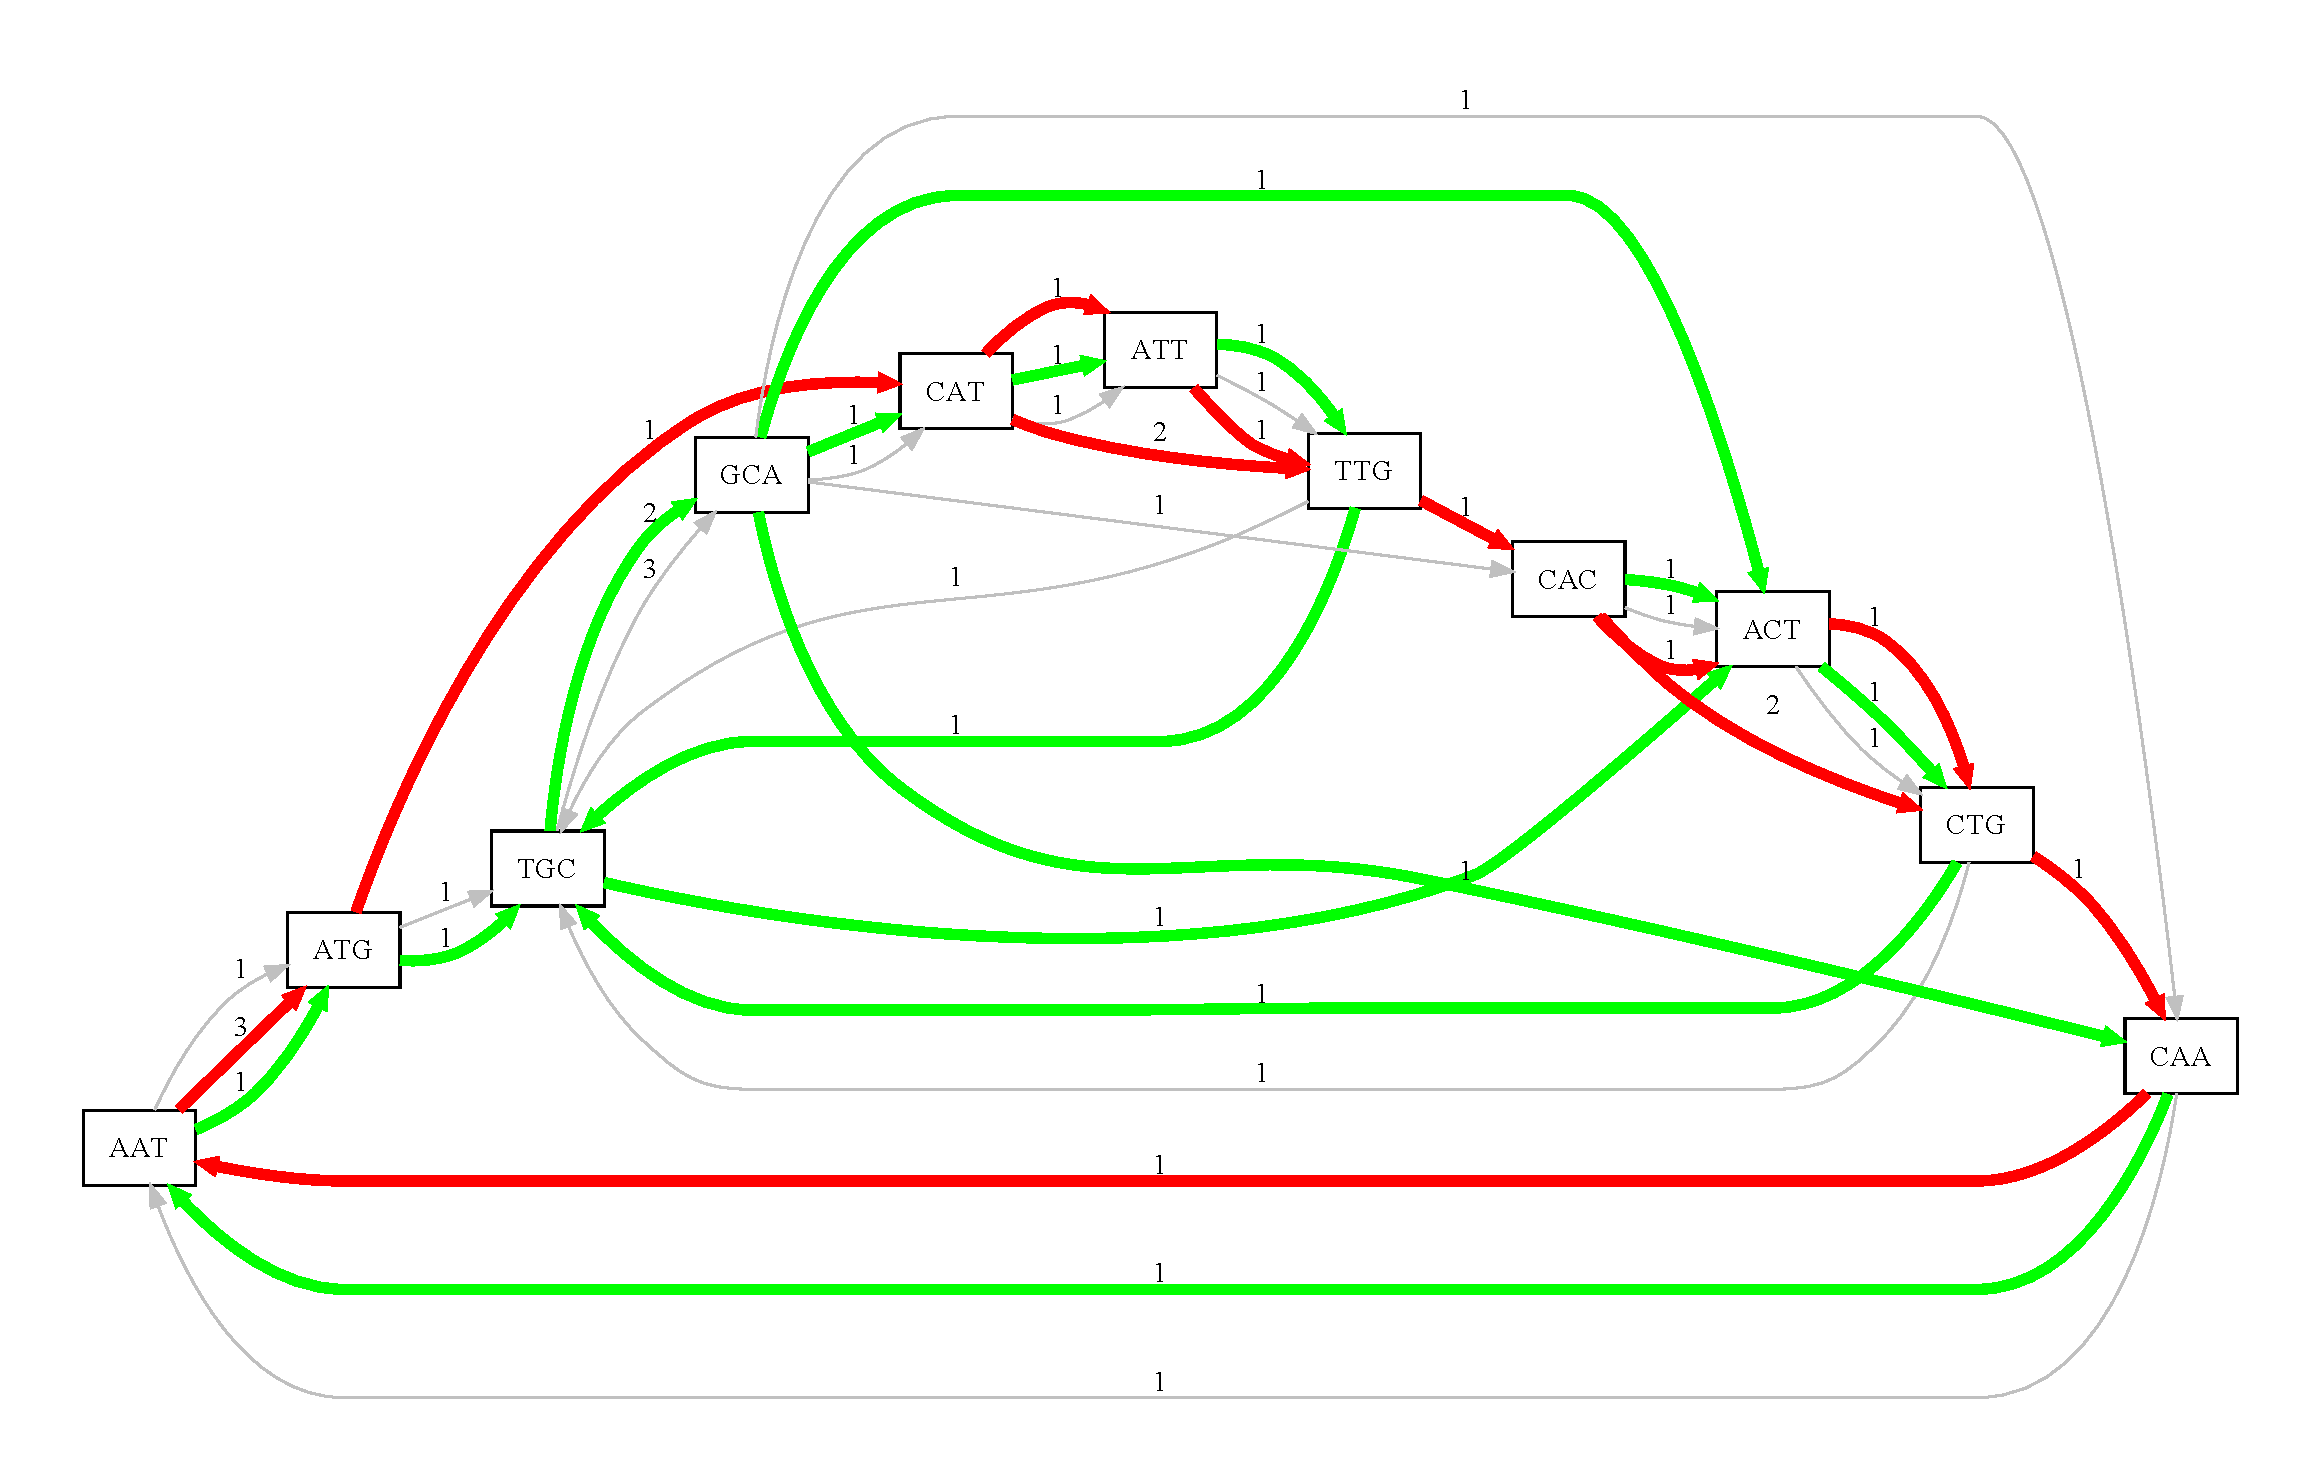
\includegraphics[width=0.9\textwidth]{TAAACGAAAC.pdf}
\end{center}
\end{figure}

\begin{figure}
\caption{A Bruijn graphs of genome {\tt ATGCATTGCACTGCA} ($readsize=6$, $k=3$)
for different orderings on $3$-mers.}\label{fig:different_orderings2}
\begin{center}
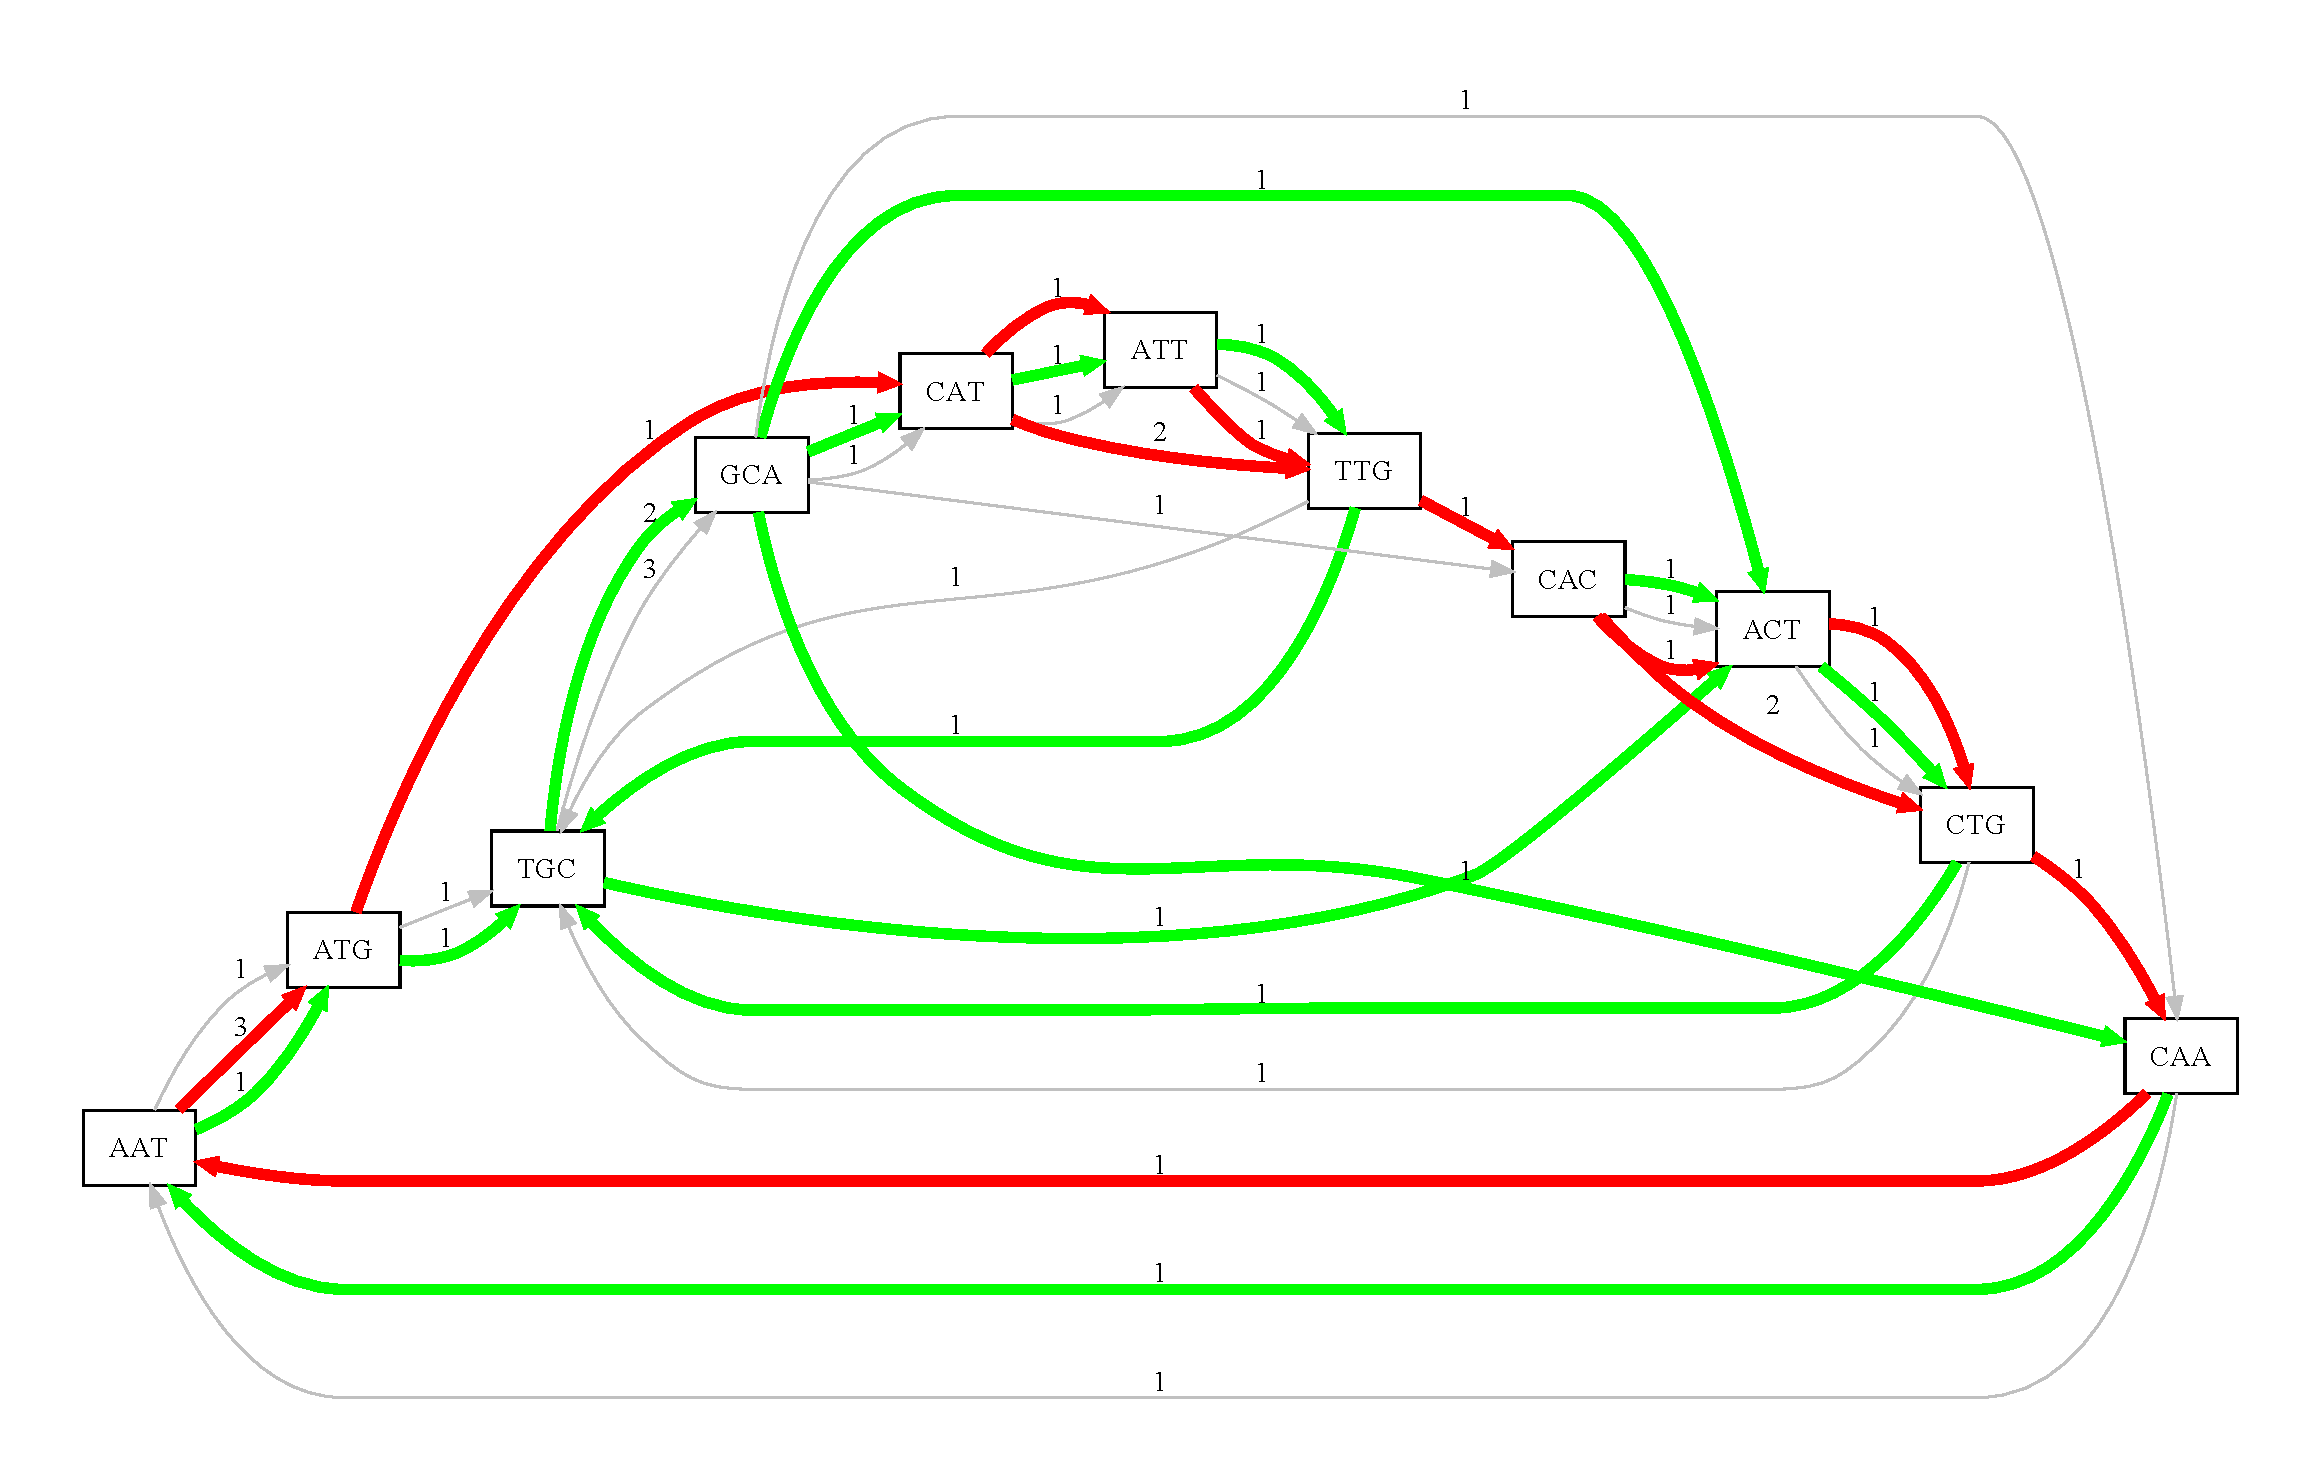
\includegraphics[width=0.9\textwidth]{ATGCATTGCACTGCA.pdf}
\end{center}
\end{figure}



\item \dots \todo{what else?..}
\end{enumerate}

\subsection{Hash Functions}

One of the possibilities to extract two distinguished $k$-mers out of a given
read is to take two $k$-mers with minimal value of some hash function $h$.
Some natural properties that $h$ should hold are listed below.
\begin{enumerate}
  \item The hash function should be easily computed.
  While iterating through all $k$-mers of a given read
  it is also important to have a fast way to recompute 
  the hash value. For this, one may take a kind of polynomial
  hash function (like in a finger-printing algorithm for the pattern 
  matching problem).
  \item It should to be stable with respect to reverse-complementary 
  $k$-mers, i.e., $h(s) = h(s^{RC})$ so that if we represent a read
  by an edge $(s_1,s_2)$, then its reverse-complement read is represented by 
  a ``reverse'' edge $(s_2^{RC},s_1^{RC})$. Two natural ways to make out a
  reverse-complementary stable hash function $h$ out of any hash function 
  $h_0$ are the following:
  \[h(s) = h_0(s) \oplus h_0(s^{RC}) \textrm{ or } h(s) = \min\{h_0(s), h_0(s^{RC})\} .\]
\end{enumerate}


The main question that still needs to be answered is:
does this graph really represent the repeat structure of the genome?

\section{Practical results}

We've implemented the suggested approach and are currently investigating the resulting A Bruijn graphs
on emulated data sets.

The technical issues pushed us towards a two-pass procedure:
\begin{enumerate}
  \item Each read undergoes a (linear-time) hashing procedure, and two least-valued $k$-mers are marked as
  ``good''. (In fact, not themselves but their hash values are marked. Even if a few extra $k$-mers become
  good due to hash collisions, it will not make much harm).
  \item For each read, all of its $k$-mers are checked whether their hash values are good, and the good ones
  are mapped to corresponding vertices in the future graph. The read is thus counted towards one or more edges.
  The leavings (in the two ends of the read) are currently not considered.
\end{enumerate}

Fig.~\ref{fig4} shows the resulting A Bruijn graph for the first 10\% of the reference E. Coli genome; the ideal data set
was used for this calculation.

\begin{figure}
\caption{10\% of E. Coli genome. $K$ = 31. Two $k$-mers from each read.}\label{fig4}
\begin{center}\includegraphics[height=0.9\textheight]{fig4.pdf}\end{center}
\end{figure}

This graph has only undergone a simple vertex-merging procedure; there are more
yet-unimplemented simplifications applicable to this graph.

\subsection{Statistics}
The plot below shows the dependence of the number of vertices in a graph from the 
number of reads for {\tt s\_6.first10000}.

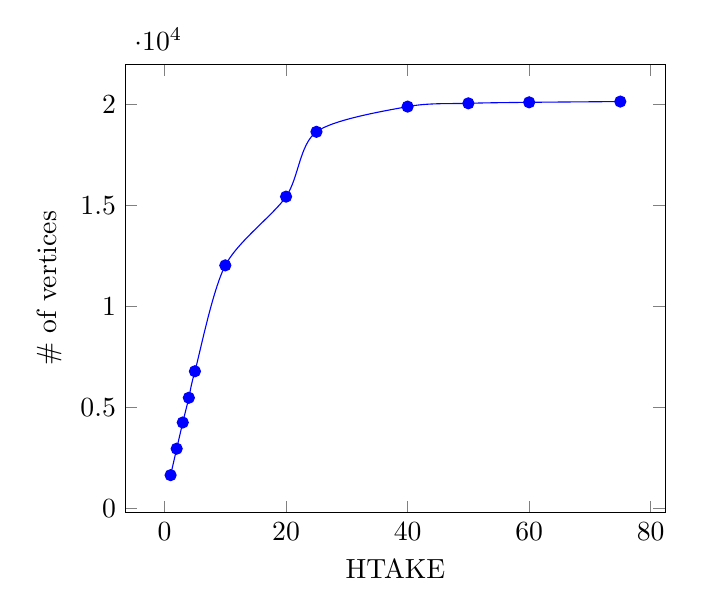
\begin{tikzpicture}
    \begin{axis}[xlabel={HTAKE},ylabel={$\#$ of vertices}]
    \addplot[smooth,mark=*,blue] plot coordinates { (1,1640) (2,2950) (3,4248) (4,5472) (5,6784)
      (10, 12028) (20, 15432) (25, 18642) (40, 19890) (50, 20052) (60, 20102) (75,20140) };
    %\addlegendentry{de Bruijn}

    %\addplot[smooth,color=red,mark=x] plot coordinates { (4000,1267) (6000,2134) (10000,5134) };
    %\addlegendentry{A Bruijn}
    \end{axis}
\end{tikzpicture}

\section{Further ideas}

\subsection{Making use of frequency}

The task of selecting the $k$-mers that will become vertices in the A Bruijn graph can be reformulated
as the task of selecting criteria that distinguish some $k$-mers among others that work the same way
in different reads.

Along with a hash function, an apt criterion is the frequency of the given $k$-mer among all reads
(provided the corresponding hash-table is memory-feasible). This criterion might be fruitful considering
the following.

\begin{itemize}
  \item The $k$-mers that are underrepresented{\todo{what do we mean by ``underrepresented''?
  is it true that most of the erroneous reads have frequency one?}} in the 
  reads (even those a with small value of hash function)
  are (most probably) erroneous. Using frequency allows us 
  to exclude them from the set of
  vertex-forming $k$-mers.
  \item The $k$-mers that are overrepresented correspond to high-degree vertices in the graph.
  It might be helpful to exclude them as well in order to make the structure of the graph more feasible.
  (Motivation: consider two reads, $axyb$ and $cxyd$. A hash function might suggest to select $k$-mers $x$ and
  $y$ which would create a fork in the graph. Selecting $a$, $b$, $c$ and $d$ on the other hand leads to
  two separate edges.)
\end{itemize}

\subsection{Reducing the number of vertices}
As said in the beginning the main motivation for considering such graphs
is that they contain fewer edges than the original de Bruijn graph. Clearly, the number of edges in the
A Bruijn graph is also reduced (the vertices with no bold adjacent edges actually do not belong
to A Bruijn graph). In order to further reduce the number of vertices we can do the following.
First, mark just one $k$-mer in each read with the minimal possible hash value. If it turned out to be
the first or the last $k$-mer of the current read, mark one more $k$-mer with the next smallest hash 
value.

In the ideal case when each possible read is present in the set of reads, this guarantess that
at least two $k$-mers will be marked in each read.
In real situations it would be reasonable to take the second $k$-mer if the first one
falls into on of the leftmost or rightmost $\tau$ positions for some treshold $\tau$.

\subsection{Paired reads}

Each single read provides one or several edges with the information of the following kind:
the two end-vertices of this edge are likely to be present in the desired graph traversal
at the distance exactly $d$ from each other.

Meanwhile, paired reads provide the information of the similar kind, but with the distance
known approximately instead of exactly.
It is a question of a separate investigation whether the approximate distances known from
paired reads is helpful when traversing an A Bruijn graph.


\section{Pseudocode of the assembler}

\todo[inline]{add high-level description of the assembler}

Iterative procedure for selecting the set of earmarked $k$-mers is the following:

\begin{enumerate}
\item From each read, select $t$ minimum hash values of its $k$-mers, add them to the global set of earmarked hash values.
\item (if $t=1$) For each read that has only one k-mer with earmarked hash value, earmark one more k-mer from this read.
\item In each read, select $k$-mers that have their hash values earmarked.
For corresponding vertices in the resulting A Bruijn graph, add all pairwise edges, storing their lengths.
For each k-mer, mark whether we've seen any $k$-mer to the left from it, and to the right.
\item For each $k$-mer that has no left or right neighbours, find a neighbour on the corresponding side
that has the smallest hash value and earmark it.
\item Repeat the previous step to minimize the number of neighbourless $k$-mers.
\end{enumerate}

\section{Schedule}
\begin{description}
  \item[April 15] implement earmarking procedure
  \item[April 18] test earmarking procedure on real data, get general statistics
  \item[April 20] test different hashing parameters on real data
  \item[April 22] implement frequency-dependent heuristics
%  \item[April 17] test graph condensation on real data
%  \item[April 30] research into the effects of different hash functions 
%  used to take minimizers
%  \item[May 10] compare the resulting A Bruijn graph with the condensed de 
%  Bruijn graph
%  \item 
\end{description}



\end{document}
